\section{Existing Bayesian coresets}
\label{sec:bayesian-coresets}

Our goal is to approximate expectations under a density $\pi(\theta)$, 
 \mbox{$ \theta \in \Theta $} expressed as the product of $N$ potentials 
$ (f(x_n, \theta))_{n=1}^{N} $ and a base density $ \pi_0(\theta)$:
\[
\pi(\theta) &\defined \frac{1}{Z} \exp \left(\sum_{n=1}^{N} f(x_n, \theta)\right) \pi_0(\theta).\label{eq:posterior}
\]
In the setting of Bayesian inference with conditionally independent data, 
the potentials are data log-likelihoods, \ie~$f(x_n, \theta) := \log \pi(x_n | \theta)$,
 $\pi_0$ is the prior density, $\pi$ is the posterior, 
and $Z$ is the marginal likelihood of the data. 
Rather than working directly with $\pi(\theta)$ for 
posterior inference---which requires a $\Theta(N)$ computation per evaluation---a
Bayesian coreset approximation of the form
\[
\pi_w(\theta) \defined \frac{1}{Z(w)} \exp\left(\sum_{n=1}^N w_n f(x_n, \theta)\right)\pi_0(\theta)
\]
for $w\in\reals^N$, $w\geq 0$ may be used in most popular posterior inference schemes~\citep{neal11,kucukelbir17,ranganath14}. If the number of nonzero entries $\|w\|_0$ of $w$ is small, this results in a significant reduction in computational burden.
Recent work has formulated the problem of constructing a  Bayesian coreset of size $M\in\nats$ as sparse variational inference~\citep{campbell19neurips},
\[
& w^\star = \argmin_{w\in\reals^N} \kl{\pi_w}{\pi}\label{eq:coresets-vi} \quad \quad
 \text{s.t.} \quad w \geq 0, \; \|w\|_0 \leq M,
\]
and showed that the objective can be minimized using stochastic estimates of $\nabla_w\kl{\pi_w}{\pi}$
based on samples from the coreset posterior $\pi_w$. 

\subsection{High-dimensional data}
\label{sec:high_dimensional_data}




Coresets, as formulated in~\cref{eq:coresets-vi}, are limited to using the
original datapoints themselves to summarize the whole dataset.
\cref{prop:original_coreset_fails} shows that this is problematic when
summarizing high-dimensional data; in the common setting of posterior inference
for a Gaussian mean, the KL divergence $\kl{\pi_{w^\star}}{\pi}$ of the
\emph{optimal} coreset of any size scales with the dimension of the data.  The
proof may be found in~\cref{app:proofs-of-failure}.
\bnprop \label{prop:original_coreset_fails}
Suppose we use $(X_n)_{n=1}^N \distiid \distNorm(0, I)$ in $\reals^d$ to perform posterior inference in a Bayesian model
with prior 
$\mu \dist \distNorm(0, I)$ and likelihood
$(X_n)_{n=1}^N  \distiid \distNorm(\mu, I).$
Then $\forall M < d$ and $\delta \in[0, 1]$, 
with probability at least $1-\delta$ the optimal size-$M$ coreset $w^\star$ satisfies
\[
\kl{\pi_{w^\star}}{\pi} \geq \frac{1}{2}\frac{N-M}{1+N}F_{d-M}^{-1}\left(\delta{N\choose M}^{-1}\right),
\]
where $F_{k}$ is the CDF of a $\chi^2$ random variable with $k$ degrees of freedom.
\enprop

The bound in~\cref{prop:original_coreset_fails} depends on $d$ through the
$\chi^2$ distribution inverse CDF. Although difficult to see directly, the
bound is reasonably large for typical values of $N, M, d, \delta$, and
increasing linearly in $d$; \cref{fig:klbound} visualizes the value of the
lower bound as a function of dimension $d$ for various coreset sizes $M$. Note
that the above bound requires the data to be high-dimensional such that $d >
M$; if $d\leq M$ the proof technique used in~\cref{app:proofs-of-failure} results in a vacuous
$\kl{\pi_{w^\star}}{\pi} = 0$ lower bound. 


\captionsetup[subfigure]{labelformat=empty}
\begin{figure}[t!]
	\centering 
	\begin{subfigure}[b]{.45\textwidth} 
		\scalebox{1}{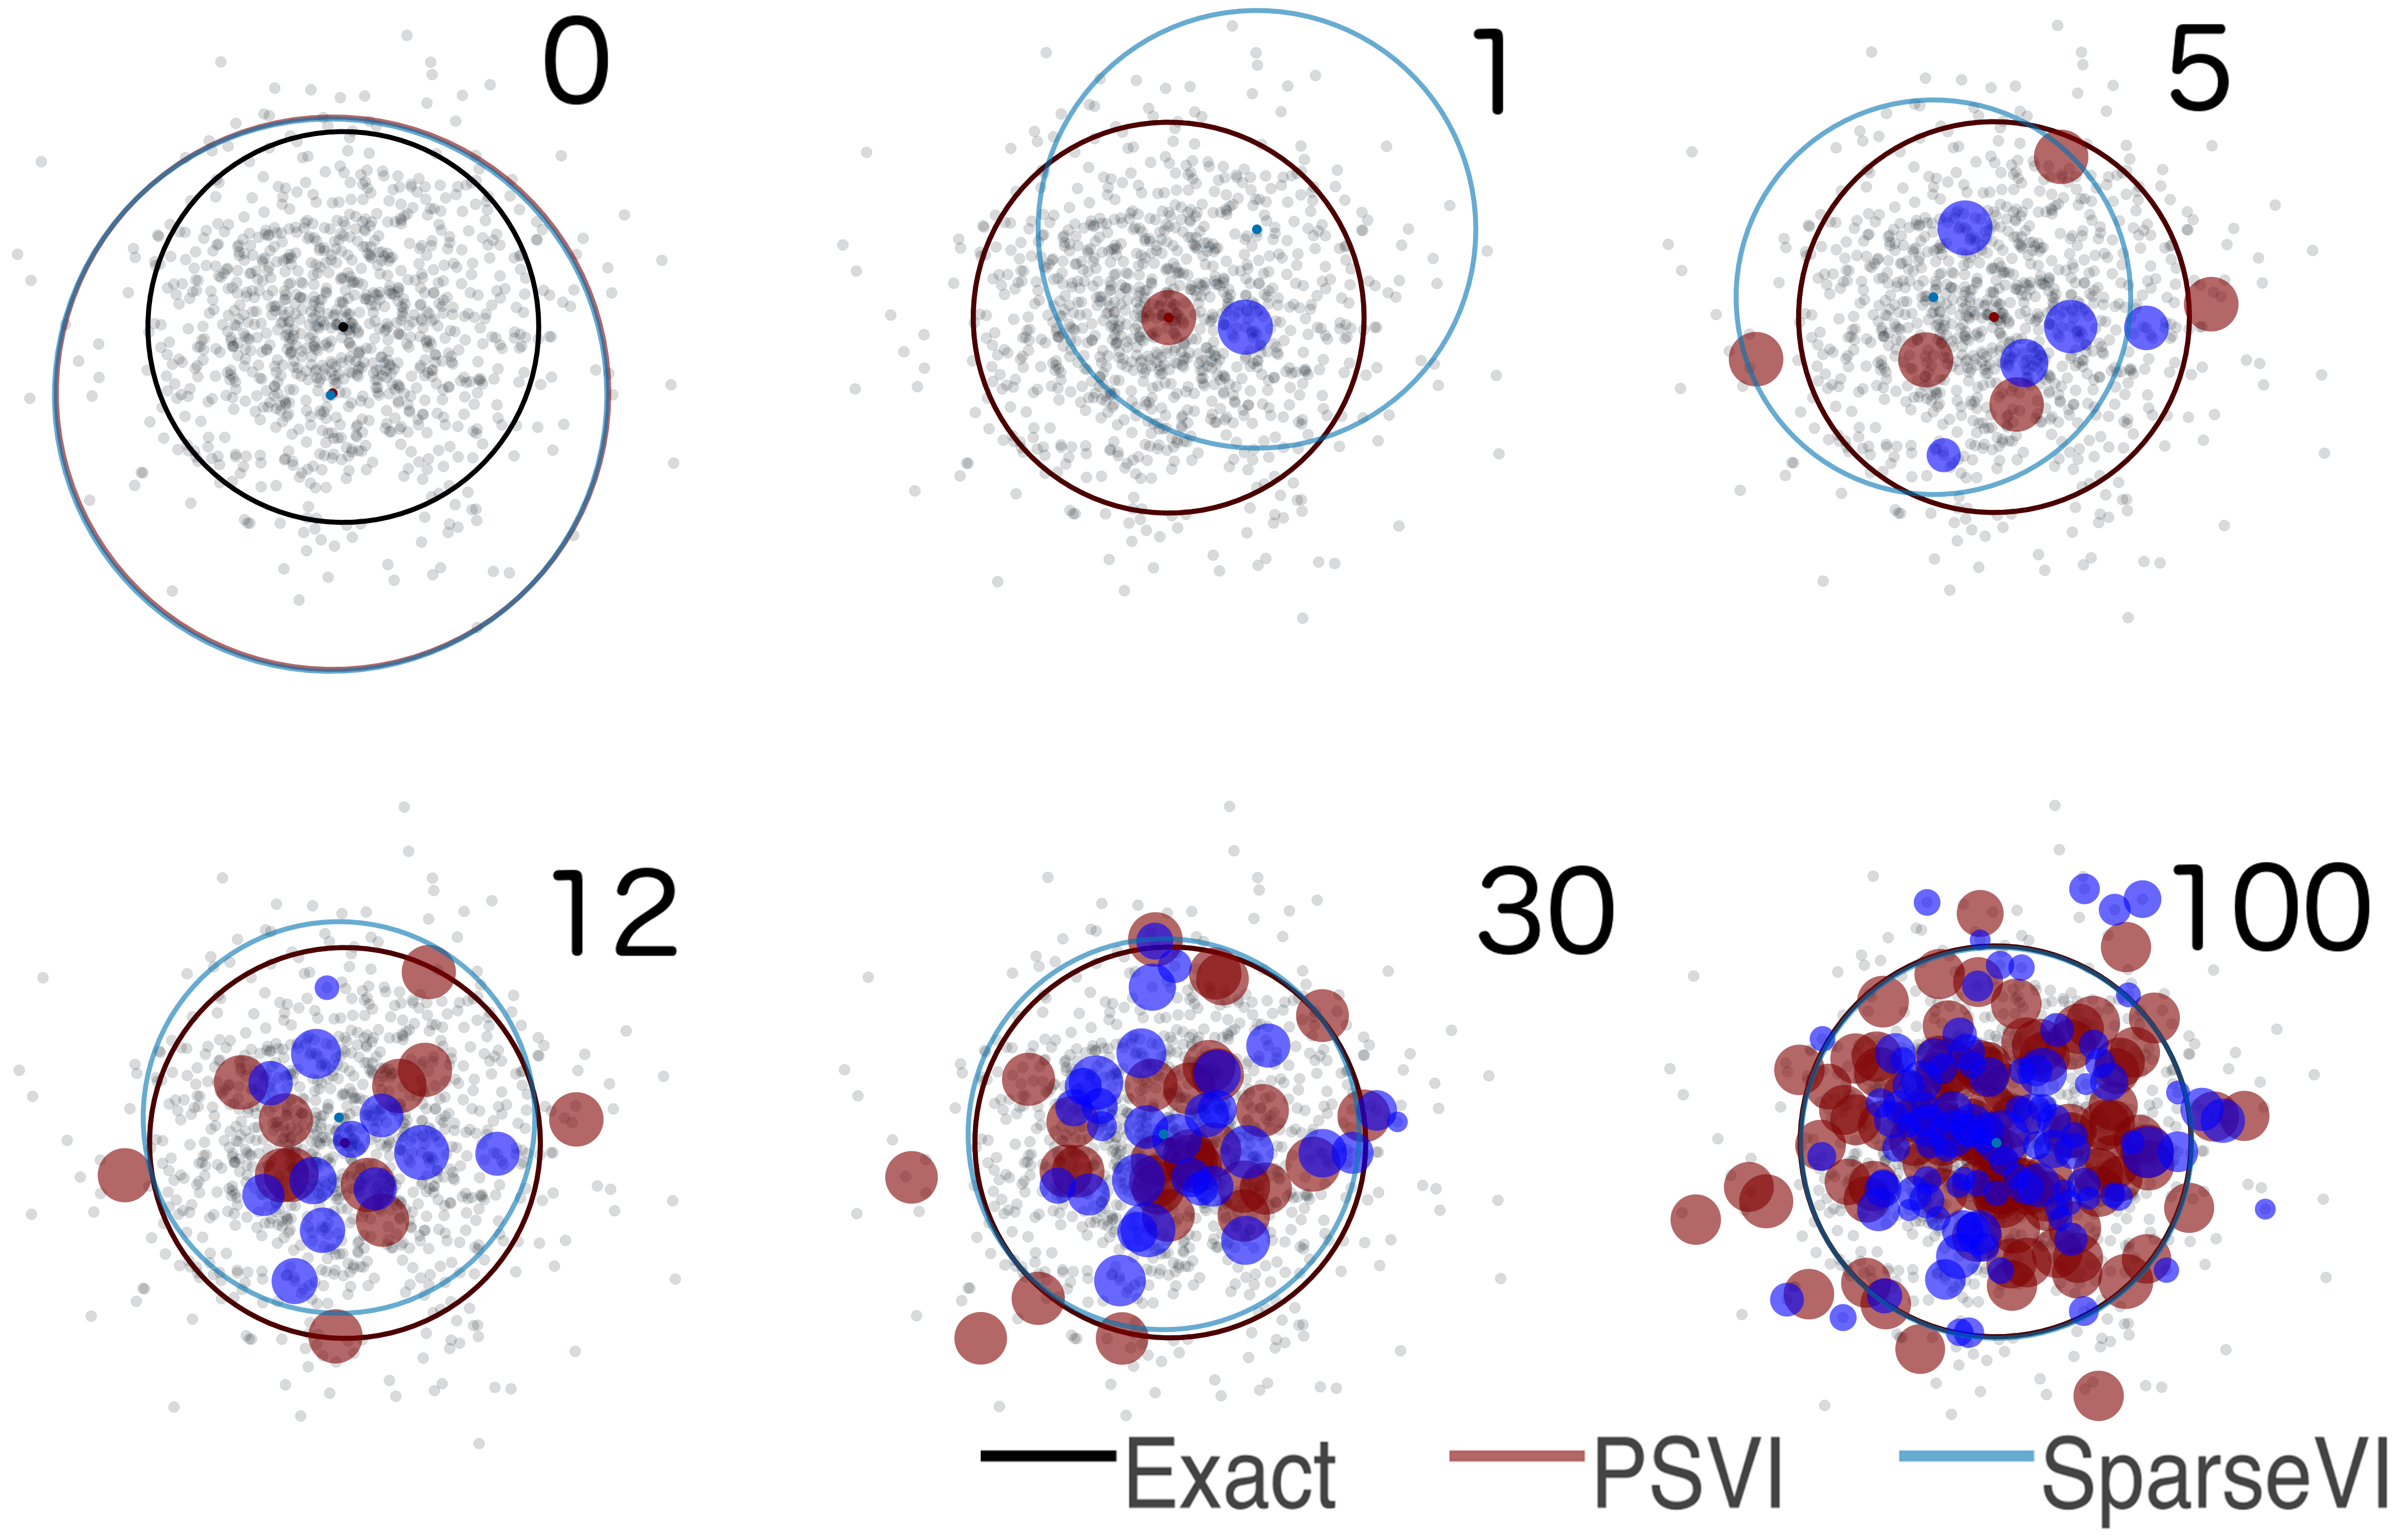
\includegraphics[width=\textwidth]{\MyPath/figs/d500_pts_combined.png}}
		\caption{(a)\label{fig:gaussian_coreset_points}}
	\end{subfigure}
	\hfill\qquad
	\centering
	\begin{subfigure}[b]{0.45\textwidth}
		\scalebox{1}{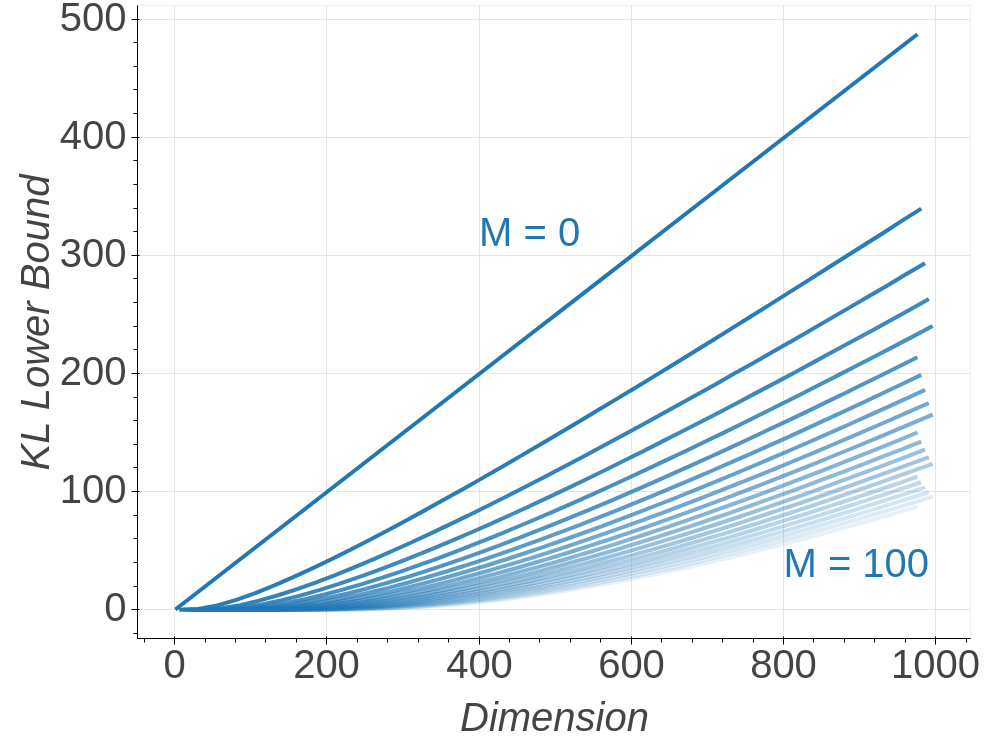
\includegraphics[width=\textwidth]{\MyPath/figs/klbound.png}}
		\caption{(b)\label{fig:klbound}}
	\end{subfigure}
	\caption{Gaussian mean inference under~pseudocoreset (\psvi)~against~standard coreset (\sparsevi) summarization for $N=1,000$  datapoints. (\subref{fig:gaussian_coreset_points})~Progression of~\psvi~vs.~\sparsevi~construction for coreset sizes $M=0, 1, 5, 12, 30, 100$, in 500 dimensions~(displayed are datapoint projections on 2 random dimensions).~\psvi~and~\sparsevi~coreset predictive $3\sigma$ ellipses are displayed in red and blue respectively, while the true posterior $3\sigma$ ellipse is shown in black.~\psvi~has the ability to immediately move pseudopoints towards the  true posterior mean, while \sparsevi~has to add a larger number of existing points in order to obtain a good posterior approximation. See \cref{fig:gauss_mean_500} for the quantitative KL comparison.
		(\subref{fig:klbound})~Optimal coreset KL divergence lower bound from \cref{prop:original_coreset_fails} as a function of dimension with $\delta = 0.5$, and  coreset size $M$ evenly spaced from 0 to 100 in increments of 5.}
\end{figure}

